\pdfoutput=1
\documentclass[11pt]{article}

\makeatletter
\def\input@path{{acl_style/}}
\makeatother
\usepackage[review]{acl}

\usepackage{booktabs}
\usepackage{multirow}
\usepackage{times}
\usepackage{latexsym}
\usepackage[T1]{fontenc}
\usepackage[utf8]{inputenc}
\usepackage{microtype}
\usepackage{graphicx}
\usepackage{amsmath}
\usepackage{enumitem}

\title{RevTrack: Evaluating Whether Scientific Assistants Know When a Review Concern Has Been Fixed}

\author{Anonymous EMNLP Submission}

\begin{document}
\maketitle

\begin{abstract}
Scientific review assistance requires temporal judgment: after authors revise a paper, a useful assistant must decide whether an old reviewer concern is still valid, partially addressed, or obsolete.
Existing review-assistance evaluations mostly score static critiques and therefore miss this revision-aware capability.
We introduce \textsc{RevTrack}, an issue-level benchmark that aligns a review concern with author response and revision evidence, then asks whether the concern is \textit{fixed}, \textit{partially fixed}, \textit{unresolved}, or \textit{regressed}.
On a hardened ICLR 2024 benchmark, a structured revision-evidence model reaches 0.704 macro-F1, compared with 0.389 for the strongest semantic encoder baseline.
On ICLR 2025, a stress set and an 80-row standard-labeled active frontier show that cross-year transfer remains brittle: TF-IDF collapses to zero fixed-case F1, and the best expanded-frontier macro-F1 is 0.469.
A user-confirmed 80-row NeurIPS 2024 active frontier adds a second venue axis: the best transferred semantic encoder reaches 0.348 macro-F1, while prompted LLMs and vote ensembles remain near majority on this frontier.
RevTrack reframes scientific review assistance as longitudinal evidence tracking and ships with auditable construction artifacts for blind validation, leakage control, label evidence, and claim readiness.
\end{abstract}

\section{Introduction}

Large language models are increasingly used as research assistants: they summarize papers, draft reviews, suggest experiments, and help authors revise manuscripts.
For these systems, static critique is not enough.
A scientifically useful assistant must update its judgment when the paper changes.
If a reviewer originally asked for computational-cost evidence and the revision adds a direct cost comparison, then repeating the old criticism is no longer helpful.
Conversely, a long and polite author response does not mean the concern was actually fixed.

\begin{figure*}[t]
\centering
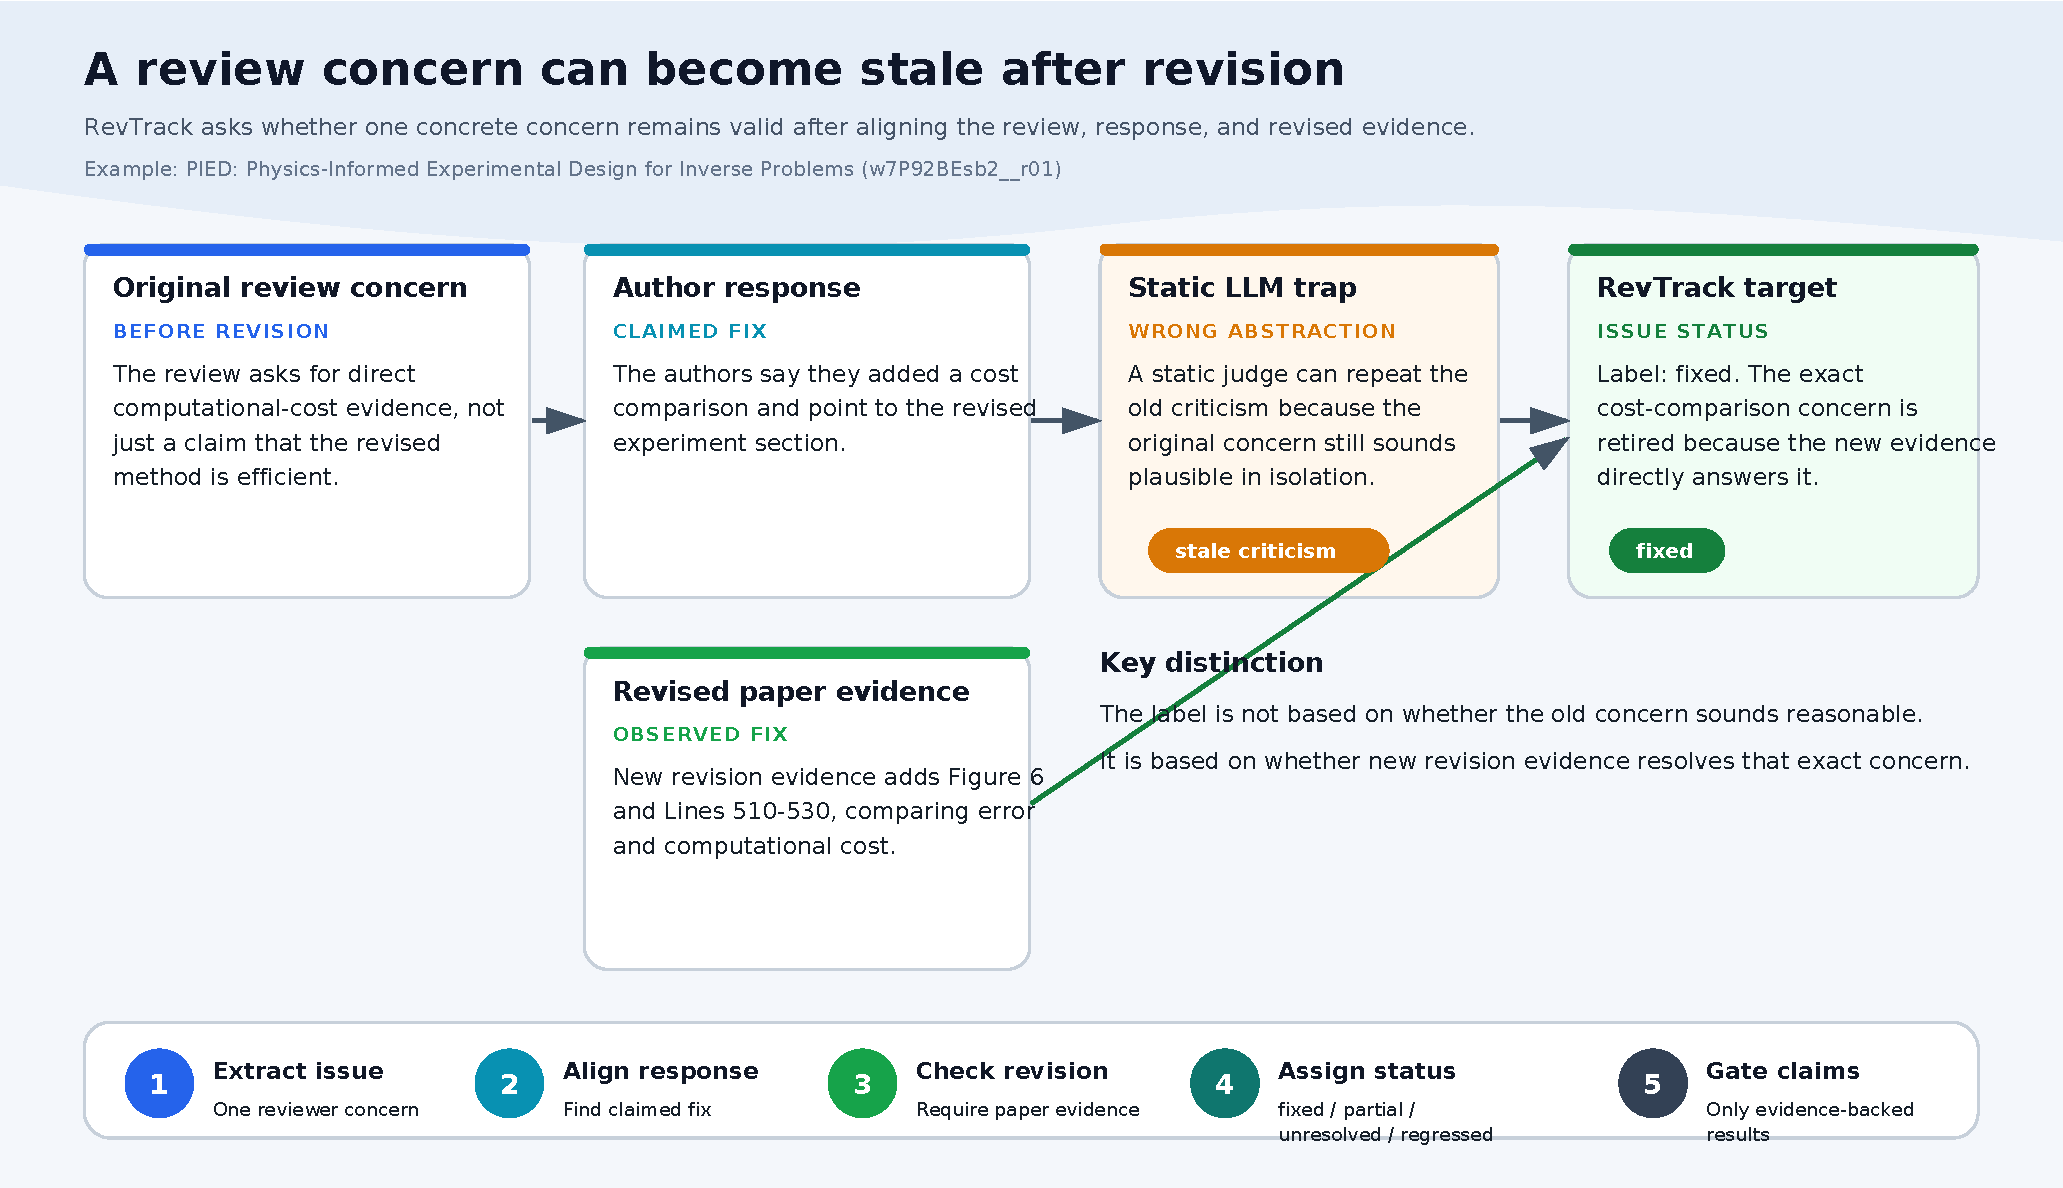
\includegraphics[width=\textwidth]{figures/figure1_revision_tracking.pdf}
\caption{RevTrack exposes a temporal failure mode: a criticism that is valid before revision can become stale after new evidence is added. The benchmark aligns each concern to the author response and revised-paper evidence before assigning an issue status, preventing static assistants from repeating obsolete criticism.}
\label{fig:running-example}
\end{figure*}

This paper studies revision-status tracking: given a paper context, one reviewer concern, author response evidence, and a revision summary, predict whether the original concern is \textit{fixed}, \textit{partially fixed}, \textit{unresolved}, or \textit{regressed}.
The task targets an evaluation blind spot.
Many review-assistance evaluations ask whether a model can produce plausible critiques, answer reviewer questions, or rate paper quality.
Those settings do not measure whether the model can maintain a structured memory of scientific concerns across revision.
As a result, systems can appear competent while still failing at the workflow that matters to authors, reviewers, and program chairs: deciding which concerns remain unresolved after the evidence changes.

We introduce \textsc{RevTrack}, a benchmark and diagnostic suite for revision-aware scientific judgment.
RevTrack builds issue-level examples from public OpenReview discussions, prioritizes hard cases with model disagreement, and keeps blind validation sheets separate from assistant/model keys.
The benchmark is organized around evidence rather than surface plausibility: each label must be supported by a review concern span, a response or revision evidence span, and a short boundary note.
The current standard validation set covers 301 audit rows across ICLR 2024, ICLR 2025, NeurIPS 2024, and ICLR 2023.
It includes 80-row active frontiers for ICLR 2025 and NeurIPS 2024, plus an 80-row ICLR 2023 random/stratified slice; all standard rows have complete evidence spans.

The empirical picture is deliberately diagnostic rather than model-chasing.
On the hardened ICLR 2024 clean-dev benchmark, a structured evidence model reaches 0.704 macro-F1, compared with 0.389 for the strongest semantic encoder baseline.
At the same time, cross-year transfer exposes brittleness.
On the ICLR 2025 stress set, a TF-IDF model matches the majority baseline in accuracy while assigning zero F1 to fixed cases.
On the standard-labeled expanded80 frontier, the best model reaches only 0.469 macro-F1; structured transfer over-credits unresolved concerns in 66 cases, while TF-IDF misses all fixed and regressed examples in that frontier.
On the user-confirmed NeurIPS 2024 active frontier, the best transferred semantic encoder reaches 0.348 macro-F1, while prompted LLMs and calibrated votes remain near the majority reference.
The ICLR 2023 random/stratified slice adds bounded external-validity evidence outside disagreement-focused active frontiers while preserving the same no-IAA and no-natural-prevalence boundary.

The central contribution is therefore not a new state-of-the-art review model.
\textsc{RevTrack} argues that the community is measuring the wrong capability for scientific assistants.
A useful assistant must not merely produce a plausible static review; it must track evidence over time, retire stale criticism, resist superficial reassurance, and flag regressions when revision makes a concern worse.
To make these claims auditable, the release includes packet-integrity checks, leakage controls, label-evidence audits, a failure taxonomy, and a claim ledger that blocks overclaiming.

Our contributions are:
\begin{itemize}[leftmargin=*]
\item We define revision-status tracking as an issue-level task for scientific review assistance.
\item We release a reproducible construction and validation pipeline with blind/key separation, evidence-span auditing, leakage checks, and claim-readiness gates.
\item We provide a validated ICLR 2024 benchmark slice, a 21-row ICLR 2025 stress set, 80-row user-confirmed active frontiers for ICLR 2025 and NeurIPS 2024, and an 80-row ICLR 2023 random/stratified standard slice.
\item We show that semantic baselines can look reasonable by accuracy while failing fixed, unresolved, and regressed-case recovery.
\item We demonstrate that structured revision evidence improves in-domain macro-F1 and use prompted LLMs, vote ensembles, and a failure taxonomy to explain where transfer models still break.
\end{itemize}

\section{Task Definition}

\paragraph{Input.}
Each example contains a paper title and optional abstract, one reviewer concern, author response candidates, an aligned response excerpt, and a revision summary.
The unit of prediction is a single issue, not a paper-level decision.
This design prevents a model from hiding behind a global paper-quality judgment when one concern was fixed and another remains unresolved.

\paragraph{Output labels.}
The label set is:
\textit{fixed}, \textit{partially fixed}, \textit{unresolved}, and \textit{regressed}.
\textit{Fixed} means the exact concern is addressed with concrete revision evidence.
\textit{Partially fixed} means the revision makes real progress but leaves a material part open.
\textit{Unresolved} means the concern remains present, is deferred, or is reframed without enough evidence.
\textit{Regressed} means the attempted fix introduces a new issue on the same axis or makes the paper less reliable.

\paragraph{Adjudication protocol.}
To reduce ambiguity at the fixed/partial/unresolved boundary, we apply the same decision order for every row.
\textbf{(1) Axis match:} check whether the revision evidence addresses the same technical axis as the reviewer concern (not just tone alignment).
\textbf{(2) Materiality:} check whether the highest-impact part of the concern is resolved for scientific judgment (for example, a missing core comparison vs a minor wording tweak).
\textbf{(3) Evidence sufficiency:} require concrete revision-facing evidence (new experiment, corrected claim, revised method detail, released artifact, or explicit limitation narrowing) rather than acknowledgement-only responses.
This yields \textit{fixed} when all three checks pass, \textit{partially fixed} when axis match and partial material progress exist but a material gap remains, \textit{unresolved} when evidence is insufficient or deferred, and \textit{regressed} when the attempted fix degrades reliability on the same axis.

\paragraph{Boundary examples in main narrative.}
Two recurring boundary patterns illustrate this protocol.
\textbf{Fixed vs partially fixed:} adding one ablation requested by the reviewer can be \textit{partially fixed} if the core missing comparison remains absent, and only becomes \textit{fixed} once the requested core comparison is present with revision evidence.
\textbf{Partially fixed vs unresolved:} a detailed rebuttal that promises future experiments remains \textit{unresolved} without revision evidence, while a partial empirical addition that narrows but does not close the concern is \textit{partially fixed}.
Appendix Table~\ref{tab:worked-issue-examples} provides compact concern/evidence snippets for all four labels.

\paragraph{Evaluation.}
Macro-F1 is the primary metric because label skew is central to the task.
Accuracy is reported only with null baselines and per-label recovery.
We explicitly track fixed-case and unresolved-case F1 because stale criticism and over-crediting are the most consequential failures for review support.

\section{Benchmark Construction}

RevTrack uses a staged construction pipeline.
First, we collect public OpenReview submissions and discussion notes \citep{openreview}.
Second, we extract issue candidates from review fields such as weaknesses, questions, and summary.
Third, we align each concern with response candidates and revision-summary text.
Fourth, we use model disagreement to prioritize hard examples.
Finally, we create blind human-validation sheets with a hidden assistant/model key and run packet integrity audits before any labels are promoted.

\begin{figure*}[t]
\centering

\includegraphics[width=\textwidth]{figures/figure_pipeline_overview.pdf}
\caption{RevTrack construction and claim-governance pipeline. The release keeps extraction quality gates, blind/key/source packet audits, label-evidence checks, and claim-readiness audits in one reproducible path so transfer claims cannot bypass provenance boundaries.}
\label{fig:pipeline-overview}
\end{figure*}

\paragraph{Example schema and leakage control.}
Each example keeps the issue identifier, paper title, review metadata, a review-concern excerpt, the top and aligned author-response excerpts, a revision summary, the status label, confidence, evidence span, and annotator note.
Blind packets omit labels, assistant suggestions, and model predictions; hidden key files retain those fields only for audit and promotion.
The packet audit checks row identity, duplicate issue identifiers, source-sheet consistency, forbidden label leakage into blind files, missing model snapshots in signoff files, and evidence-span completeness before a sheet can support a paper claim.

\begin{table*}[t]
\centering
\scriptsize
\setlength{\tabcolsep}{3pt}
\begin{tabular}{p{0.26\textwidth}rp{0.20\textwidth}p{0.36\textwidth}}
\toprule
Artifact & Rows & Status & Notes \\
\midrule
ICLR 2024 clean dev v7 & 148 & release candidate & fixed 50 / partial 86 / unresolved 11 / regressed 1 \\
ICLR 2024 train v8 & 180 & transfer training source & fixed 63 / partial 104 / unresolved 12 / regressed 1 \\
ICLR 2024 candidate pool & 230 & quality gate passed & complete rate 1.000; disagreement rows 82 \\
ICLR 2024 validation v1 & 40 & standard labels locked & user-reviewed signoff promoted on 2026-04-26 \\
ICLR 2025 repro v2 & 21 & validated stress sample & fixed 5 / partial 16 \\
ICLR 2025 expanded80 pool & 322 & construction-ready & complete rate 0.963; disagreement rows 244 \\
ICLR 2025 expanded80 validation v1 & 80 & standard labels locked & user-confirmed single-pass validation; active frontier \\
NeurIPS 2024 limit100 validation v1 & 80 & standard labels locked & user-confirmed single-pass validation; partial 44 / unresolved 36 \\
ICLR 2023 random80 validation v1 & 80 & standard labels locked & random/stratified slice; fixed 5 / partial 49 / unresolved 26 \\
\bottomrule
\end{tabular}
\caption{Current RevTrack dataset and validation artifacts. Expanded80 and NeurIPS 2024 limit100 are user-confirmed active frontiers; ICLR 2023 random80 is a user-confirmed random/stratified slice. These are not two-annotator agreement sets or venue-wide prevalence estimates.}
\label{tab:dataset-versions}
\end{table*}


\paragraph{Quality gates.}
The ICLR 2024 candidate pool contains 230 candidates with complete required text fields and 82 multi-model disagreement rows.
The expanded ICLR 2025 pool contains 322 candidates from 80 submissions, has a complete-field rate of 0.963, and includes 244 disagreement rows.
The NeurIPS 2024 limit100 candidate pool contains 393 entries with 1.000 complete-field rate and 316 disagreement rows; its 80-row active frontier is user-confirmed single-pass standard validation.
The ICLR expanded80 frontier is standard-labeled through user-confirmed single-pass validation.
The ICLR 2023 complete-field pool contains 241 candidates and 83 TF-IDF/issue-ledger disagreement rows; its 80-row random/stratified validation slice is user-confirmed single-pass standard validation.
Because the ICLR 2025 and NeurIPS 2024 frontiers are active-sampled from model disagreement, we treat them as hardened transfer frontiers rather than estimates of natural venue-level issue prevalence.
Because the ICLR 2023 slice is random/stratified rather than an active frontier, we report it by measured slice design and still avoid unmeasured natural-prevalence claims.

\paragraph{Validation provenance.}
The current standard human-validation set contains 301 rows: 40 from ICLR 2024, 21 from the ICLR 2025 repro stress set, 80 from the ICLR 2025 expanded frontier, 80 from the NeurIPS 2024 active frontier, and 80 from the ICLR 2023 random/stratified slice.
The first 61 rows were promoted after user-reviewed AI-assisted signoff on 2026-04-26; expanded80 was promoted after user-confirmed review of the assistant-adjudication draft on the same date; the NeurIPS 2024 resolved candidate was promoted after user confirmation on 2026-04-28.
The ICLR 2023 random80 slice was promoted after user confirmation on 2026-04-29.
We report this provenance explicitly.
The primary 301-row standard set remains single-user confirmed.
Separately, a bounded independent second-pass mini60 packet was completed with agreement $=1.0$, Cohen's $\kappa=1.0$, and zero mismatches.
Because mini60 is intentionally bounded and boundary-focused, we use it as protocol-consistency evidence on hard cases rather than as full-scale two-annotator coverage of all packets.
Accordingly, we do not report full-dataset inter-annotator reliability claims for the entire benchmark in this version.
The release package includes a dataset card, claim-evidence ledger, packet audits, label-evidence audits, and the scripts used to regenerate tables and figures from machine-readable CSV, JSON, TSV, and JSONL artifacts.

\section{Baselines and Diagnostic Models}

We compare three families of models.
\textbf{Null baselines} predict the majority label, primarily to expose the accuracy trap under skew.
\textbf{Semantic baselines} train TF-IDF or encoder representations with a linear classifier.
They test whether issue resolution can be recovered from generic text similarity.
\textbf{Structured diagnostic models} expose evidence slots and follow-up cues to a calibrator.
This model is deliberately simple: its purpose is to test whether revision-specific structure helps, not to maximize architecture novelty.

The issue-ledger and structured calibrator are designed as diagnostic interventions.
They encode cues such as concrete added experiments, softened claims, future-work deferrals, and response-only fixes.
Hard overrides are reported with an ablation so that the gain from explicit revision cues is visible.

\paragraph{Structured feature groups.}
The structured calibrator uses only observable fields from the issue sheet: request type cues in the review concern, response/revision cues for added evidence, broad-evaluation responses, theory or notation fixes, code-release promises, future-work deferrals, digit/count buckets, and the disagreement pattern among semantic baselines.
It also includes an issue-ledger label and rule as diagnostic features.
For ICLR 2024 clean-dev evaluation, we use leave-one-out training: each row is predicted by a classifier trained on all other labeled rows, with hard overrides disabled in the ablation row.
Transfer predictions train on the frozen labeled source sheet and are never used as labels for blind validation packets.

\section{Experiments}

The experiments ask whether systems can update a concrete review issue after revision evidence, not merely whether they can produce plausible criticism.
We therefore read every result through two lenses: macro-F1 and per-label recovery under skew, and the failure modes in Table~\ref{tab:failure-taxonomy}.
The first two RQs quantify the accuracy trap; the latter two explain what breaks when models transfer across years.
Across all splits, three findings persist: (i) structured evidence gives the clearest in-domain gain, (ii) accuracy alone hides severe label-level failures, and (iii) prompted transfer remains brittle even with model voting and calibration rules.

\subsection{RQ1: Does Structure Help In Domain?}

\begin{table}[t]
\centering
\scriptsize
\setlength{\tabcolsep}{3pt}
\begin{tabular}{p{0.42\linewidth}rrr}
\toprule
Model & Accuracy & Macro-F1 & Fixed F1 \\
\midrule
Majority label & 0.581 & 0.184 & 0.000 \\
TF-IDF + LinearSVC & 0.561 & 0.376 & 0.510 \\
ModernBERT & 0.561 & 0.387 & 0.509 \\
MPNet & 0.581 & 0.389 & 0.554 \\
Structured without hard rules & 0.655 & 0.424 & 0.602 \\
Structured & \textbf{0.682} & \textbf{0.704} & \textbf{0.624} \\
\bottomrule
\end{tabular}
\caption{ICLR 2024 clean dev v7 results. Macro-F1 is the primary metric because label skew makes accuracy misleading.}
\label{tab:main-results}
\end{table}


Table~\ref{tab:main-results} shows that structured revision evidence substantially improves macro-F1 on ICLR 2024 clean dev v7.
The strongest semantic baseline, MPNet with a linear classifier, reaches 0.581 accuracy and 0.389 macro-F1.
The structured model reaches 0.682 accuracy and 0.704 macro-F1.
Removing structured hard overrides drops macro-F1 to 0.424, showing that explicit revision-follow-up cues drive much of the minority-label recovery.
This large drop also clarifies the model role: the strongest in-domain system is a diagnostic hybrid that combines learned scoring with benchmark-specific explicit cues.

\subsection{RQ2: When Does Accuracy Mislead?}

\begin{table}[t]
\centering
\scriptsize
\setlength{\tabcolsep}{3pt}
\begin{tabular}{p{0.18\linewidth}p{0.22\linewidth}rrr}
\toprule
Dataset & System & Accuracy & Macro-F1 & Fixed F1 \\
\midrule
ICLR 2024 & Majority & 0.581 & 0.184 & 0.000 \\
ICLR 2024 & TF-IDF & 0.561 & 0.376 & 0.510 \\
ICLR 2025 & Majority & 0.762 & 0.216 & 0.000 \\
ICLR 2025 & TF-IDF & 0.762 & 0.216 & 0.000 \\
\bottomrule
\end{tabular}
\caption{Null-baseline comparison. On the ICLR 2025 stress set, TF-IDF matches the majority baseline while failing fixed-case recovery.}
\label{tab:null-baselines}
\end{table}


Table~\ref{tab:null-baselines} shows why accuracy is insufficient.
On ICLR 2024, the majority-label baseline reaches the same accuracy as the best semantic baseline but has zero F1 for fixed, unresolved, and regressed cases.
On the ICLR 2025 repro stress set, TF-IDF exactly matches the majority baseline while assigning zero F1 to fixed cases.
This is the core evaluation failure RevTrack is designed to surface.

\subsection{RQ3: What Fails Qualitatively?}

The failure taxonomy is the bridge from aggregate scores to reviewer-facing risk and is a primary claim-bearing result, not an auxiliary error list.
It identifies five recurring modes.
\textit{Stale criticism} occurs when a model preserves an old concern after direct revision evidence fixes it.
\textit{Over-crediting} occurs when a long response acknowledges a limitation without resolving it.
\textit{Fixed under-recovery} occurs when the model keeps a resolved concern alive because the original critique remains lexically salient.
\textit{Partial-fix ambiguity} occurs when added evidence narrows but does not eliminate the concern.
\textit{Regression scarcity} remains a limitation: the current clean-dev pool contains only one regressed example, so regression performance is not yet a stable claim.
Table~\ref{tab:failure-taxonomy} turns these modes into paper-facing evidence rather than a post-hoc error list.
On expanded80, the structured transfer model over-credits unresolved concerns as fixed or partially fixed in 66 cases, TF-IDF misses all four fixed examples and all six regressed examples, and the strongest issue-ledger model still makes four partial/full-boundary errors.
These counts should be read as active-frontier diagnostics, not natural prevalence.

\begin{table}[t]
\centering
\scriptsize
\setlength{\tabcolsep}{3pt}
\begin{tabular}{p{0.22\linewidth}p{0.31\linewidth}p{0.35\linewidth}}
\toprule
Failure mode & Pattern & Evidence use \\
\midrule
Stale criticism & predicts partially\_fixed or unresolved because the original concern remains semantically plausible & This example separates revision-aware judgment from static semantic plausibility. \\
Over-crediting & over-credits unresolved concerns as fixed or partially fixed (66 expanded80 errors) & This is the practical stale-assistant failure: the model would stop tracking an unresolved concern. \\
Fixed under-recovery & keeps a fixed concern alive as partially fixed or unresolved (4 expanded80 errors) & This motivates fixed-case F1 rather than accuracy-only reporting. \\
Regression blindness & misses cases where the revision introduces or worsens a problem (6 expanded80 errors) & This justifies keeping the regressed label while avoiding strong regression-performance claims. \\
Partial/full boundary & collapses partial resolution into fixed (4 expanded80 errors) & This is the central label-boundary risk for benchmark reliability. \\
\bottomrule
\end{tabular}
\caption{Qualitative failure taxonomy used to interpret RevTrack errors. Expanded80 counts are from the user-confirmed standard active frontier and should not be read as natural prevalence.}
\label{tab:failure-taxonomy}
\end{table}


\begin{figure*}[t]
\centering
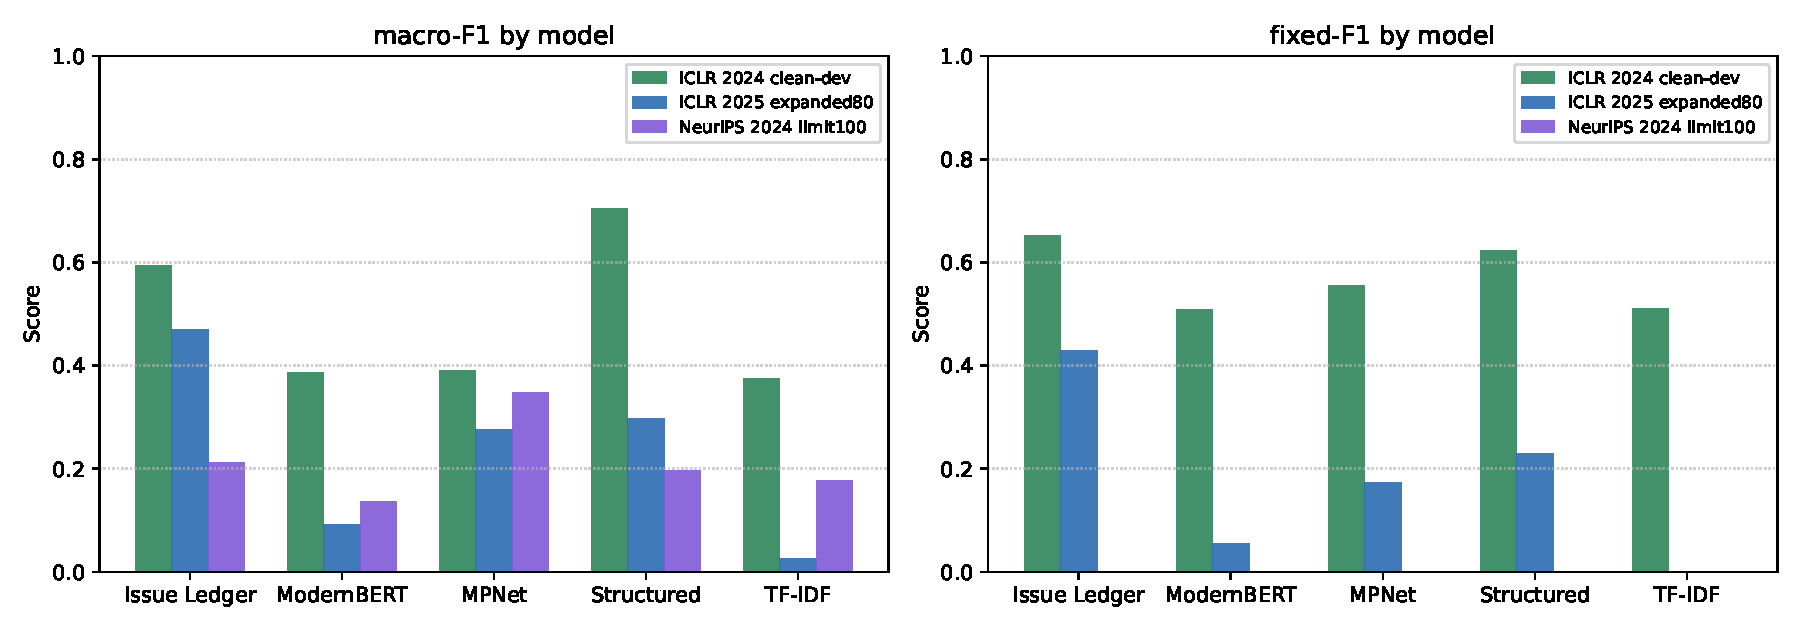
\includegraphics[width=\textwidth]{figures/figure2_transfer_breakdown.pdf}
\caption{Transfer-profile summary from three settings. Structured models and issue-ledger rules dominate in-domain and frontier settings on macro-F1, but fixed-label recovery remains weak under transfer and the NeurIPS 2024 frontier is dominated by unresolved cases.}
\label{fig:transfer-breakdown}
\end{figure*}

\subsection{RQ4: What Transfers Across Years and Venues?}

\begin{table}[t]
\centering
\scriptsize
\setlength{\tabcolsep}{3pt}
\begin{tabular}{p{0.28\linewidth}rrrr}
\toprule
Model & Accuracy & Macro-F1 & Fixed F1 & Regressed F1 \\
\midrule
TF-IDF & 0.050 & 0.026 & 0.000 & 0.000 \\
ModernBERT & 0.125 & 0.092 & 0.056 & 0.000 \\
MPNet & 0.312 & 0.276 & 0.174 & 0.500 \\
Structured & 0.150 & 0.298 & 0.229 & \textbf{0.800} \\
Issue ledger & \textbf{0.850} & \textbf{0.469} & \textbf{0.429} & 0.500 \\
\bottomrule
\end{tabular}
\caption{ICLR 2025 expanded80 standard-labeled active frontier. The frontier is intentionally hard and model-disagreement-heavy, so it supports transfer brittleness analysis rather than natural label-prevalence estimates.}
\label{tab:expanded80-transfer}
\end{table}

\begin{table}[t]
\centering
\scriptsize
\setlength{\tabcolsep}{2pt}
\begin{tabular}{p{0.25\linewidth}ccccc}
\toprule
Model & Acc. & Macro & Fixed & Partial & Unres. \\
\midrule
Issue Ledger & 0.500 & 0.211 & 0.000 & 0.167 & 0.679 \\
ModernBERT & 0.200 & 0.137 & 0.000 & 0.229 & 0.320 \\
MPNet & 0.550 & 0.348 & 0.000 & 0.516 & 0.875 \\
Structured & 0.362 & 0.197 & 0.000 & 0.545 & 0.244 \\
TF-IDF & 0.550 & 0.177 & 0.000 & 0.710 & 0.000 \\
\bottomrule
\end{tabular}
\caption{NeurIPS 2024 limit100 user-confirmed single-pass active frontier transfer from the ICLR 2024 model stack. No fixed or regressed examples are present in this frontier, so fixed/regressed F1 are unavailable for stronger interpretation.}
\label{tab:neurips100-transfer}
\end{table}


\textbf{In-domain to ICLR 2025} is still the strongest signal for proving in-year revision-aware gain, but both expanded80 and NeurIPS limit100 are purposefully hard.
Cross-venue transfer confirms the same pattern:
high aggregate scores alone can mask clinically important misses, while unresolved concerns remain the hardest safety-critical case.

The validated ICLR 2025 repro set is a stress test, not a full benchmark.
It reveals brittleness: the majority baseline and TF-IDF both reach 0.762 accuracy, while TF-IDF has fixed-label F1 of 0.000.
The expanded ICLR 2025 frontier removes the scale blocker at the active-frontier stage: it contains 322 candidates and 244 model-disagreement rows, and its 80-row validation packet has complete standard labels and evidence spans.
Table~\ref{tab:expanded80-transfer} shows this frontier remains difficult under transfer.
Table~\ref{tab:neurips100-transfer} shows the same trend in a different venue ecology and is included as a standard single-user cross-venue active frontier.
It also shows unresolved labels still dominating and fixed recovery absent in the current split.
Issue-ledger rules are strongest overall in this bounded frontier setting, while TF-IDF and encoder baselines have weak macro-F1 and poor fixed-case recovery.
This supports a cross-year brittleness claim, but not a broad prevalence claim, because the frontier is intentionally model-disagreement-heavy.
Because these frontiers are disagreement-harvested hard subsets, they should be read as stress-test transfer evidence rather than as a full distributional estimate of venue-wide revision behavior.
The ICLR 2023 random/stratified slice complements these frontiers with 80 standard rows and a fixed/partial/unresolved label mix of 5/49/26.
It supports bounded external-validity evidence by measured slice design, not a claim about natural venue prevalence.
Appendix Table~\ref{tab:cross-split-significance} reports stratified-bootstrap confidence intervals for all three standard splits; ranking uncertainty is small for the in-domain gap and substantially larger on transfer frontiers.

\subsection{RQ5: How Do Prompted LLM Baselines Behave Under Transfer?}

\begin{table}[t]
\centering
\scriptsize
\setlength{\tabcolsep}{2pt}
\begin{tabular}{p{0.28\linewidth}cccc}
\toprule
Model & ICLR24 & ICLR25 & NeurIPS & Mean \\
\midrule
Majority & 0.184 & 0.226 & 0.177 & 0.196 \\
GPT-5.5 (v2) & 0.350 & 0.081 & 0.171 & 0.201 \\
GPT-4.1 & 0.326 & 0.070 & 0.166 & 0.187 \\
GPT-4o-mini & 0.299 & 0.077 & 0.178 & 0.185 \\
GPT-4.1-nano & 0.210 & 0.161 & 0.126 & 0.166 \\
Qwen2.5-72B & 0.334 & 0.072 & 0.165 & 0.190 \\
GPT-4.1-mini & 0.347 & 0.066 & 0.181 & 0.198 \\
\midrule
Vote-3 (top) & 0.352 & 0.071 & 0.179 & 0.201 \\
Vote-3 (diverse) & 0.347 & 0.088 & 0.174 & 0.203 \\
Vote-3 (U-guard) & 0.345 & 0.092 & 0.170 & 0.202 \\
Vote-3 (U+F) & 0.350 & 0.094 & 0.167 & 0.204 \\
Vote-6 (all) & 0.344 & 0.064 & 0.177 & 0.195 \\
\bottomrule
\end{tabular}
\caption{Macro-F1 of prompted LLMs and vote ensembles on three standard-labeled splits. Voting improves in-domain stability but does not resolve cross-year brittleness on expanded80.}
\label{tab:prompted-llm-ensemble}
\end{table}


Table~\ref{tab:prompted-llm-ensemble} adds six prompted-LLM baselines, five vote-calibration variants, and a majority-label reference on the same standard-labeled splits.
In-domain ICLR 2024 is competitive for several prompted variants, but transfer remains brittle.
On ICLR 2025 expanded80, all prompted and ensemble variants remain below the majority-label macro-F1 baseline (0.226); the strongest calibrated vote reaches 0.094.
On NeurIPS limit100, the best prompted model reaches 0.181 macro-F1, while the best vote reaches 0.179 and stays near the majority baseline (0.177).
Model pooling therefore improves stability but does not close the longitudinal transfer gap.
Appendix Table~\ref{tab:prompted-llm-bootstrap} shows the same risk under bootstrap uncertainty: ICLR24 prompted rows are above majority, ICLR25 rows remain below majority, and NeurIPS24 rows mostly overlap the majority reference.
Appendix Table~\ref{tab:prompted-llm-significance} reports paired stratified-bootstrap significance against the majority baseline: prompted rows are reliably above majority in-domain, reliably below majority on ICLR25 expanded80, and statistically overlapping on NeurIPS24.

\begin{table*}[t]
\centering
\scriptsize
\setlength{\tabcolsep}{3pt}
\begin{tabular}{lrrrrrr}
\toprule
Variant & Prompt & Temp & Accuracy & Macro-F1 & U Recall & F Recall \\
\midrule
GPT-4o-mini & default & 0.0 & 0.062 & 0.077 & 0.015 & 0.250 \\
GPT-4o-mini & default & 0.3 & 0.038 & 0.020 & 0.015 & 0.000 \\
GPT-4o-mini & default & 0.7 & 0.038 & 0.021 & 0.015 & 0.000 \\
GPT-4o-mini & unresolved-strict & 0.0 & 0.062 & 0.032 & 0.015 & 0.000 \\
GPT-5.5(v2) & default & 0.0 & 0.088 & 0.081 & 0.045 & 0.250 \\
GPT-5.5(v2) & unresolved-strict & 0.0 & 0.100 & 0.059 & 0.091 & 0.000 \\
GPT-4.1-mini & default & 0.0 & 0.062 & 0.066 & 0.015 & 1.000 \\
GPT-4.1-mini & unresolved-strict & 0.0 & 0.100 & 0.086 & 0.061 & 1.000 \\
GPT-4.1-nano & default & 0.0 & 0.350 & 0.161 & 0.379 & 0.750 \\
GPT-4.1-nano & unresolved-strict & 0.0 & 0.412 & 0.171 & 0.485 & 0.250 \\
\bottomrule
\end{tabular}
\caption{Expanded80 decoding/prompt ablation for prompted transfer. Temperature increases are uniformly harmful. Unresolved-strict prompting is model-dependent: it hurts GPT-4o-mini and GPT-5.5(v2) macro-F1, while improving GPT-4.1-mini and GPT-4.1-nano unresolved recall and macro-F1 with trade-offs on fixed recall.}
\label{tab:prompted-llm-temp}
\end{table*}


Table~\ref{tab:prompted-llm-temp} shows targeted decoding/prompt ablations on expanded80.
Raising temperature (0.0 to 0.3/0.7) lowers macro-F1 from 0.077 to around 0.020, so transfer errors are not resolved by sampling diversity.
Unresolved-strict prompting is model-dependent: it hurts GPT-4o-mini and GPT-5.5(v2), but improves GPT-4.1-mini and GPT-4.1-nano with different fixed-recall trade-offs.
Even with those gains, absolute transfer performance remains low and below the majority baseline.
Full offline calibration-rule search results are reported in Appendix Table~\ref{tab:prompted-llm-postprocess-rules}.

\begin{figure*}[t]
\centering
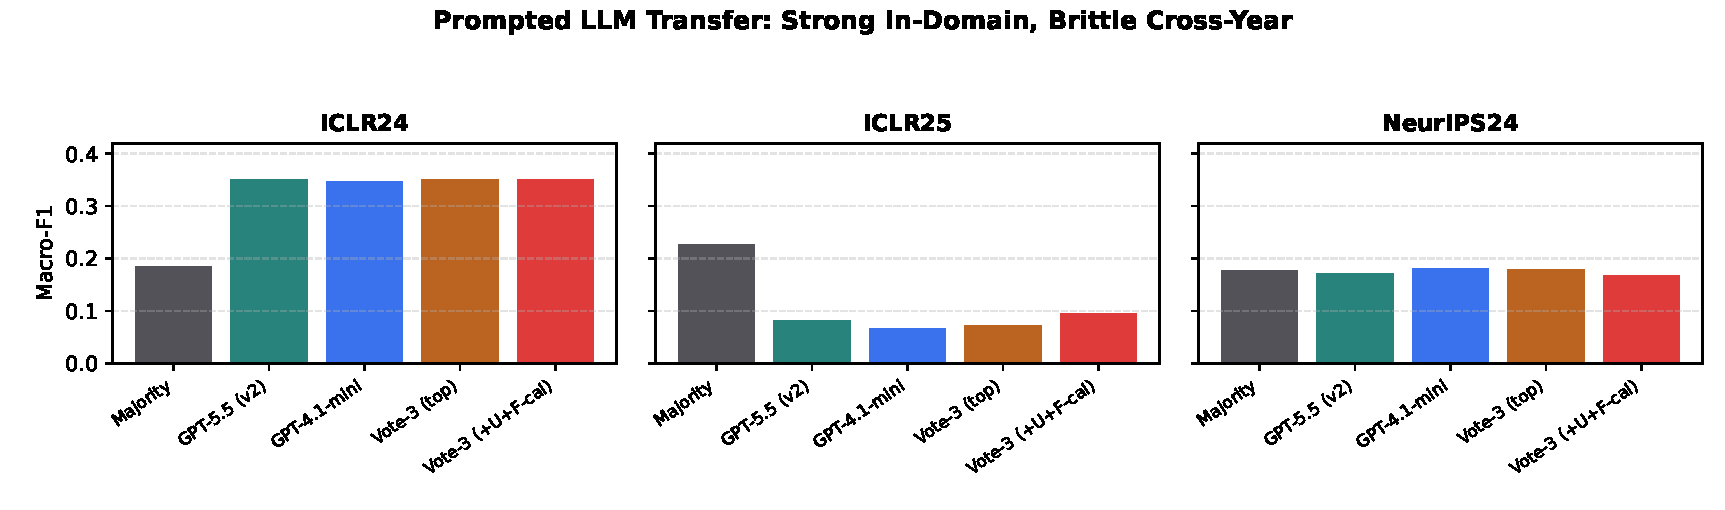
\includegraphics[width=\textwidth]{figures/figure3_prompted_llm_transfer.pdf}
\caption{Prompted-LLM transfer profile with majority baseline and vote ensembles, including calibrated unresolved/fixed safeguards. Ensemble voting improves ICLR 2024 stability but does not recover cross-year robustness on expanded80.}
\label{fig:prompted-llm-transfer}
\end{figure*}

\begin{figure*}[t]
\centering
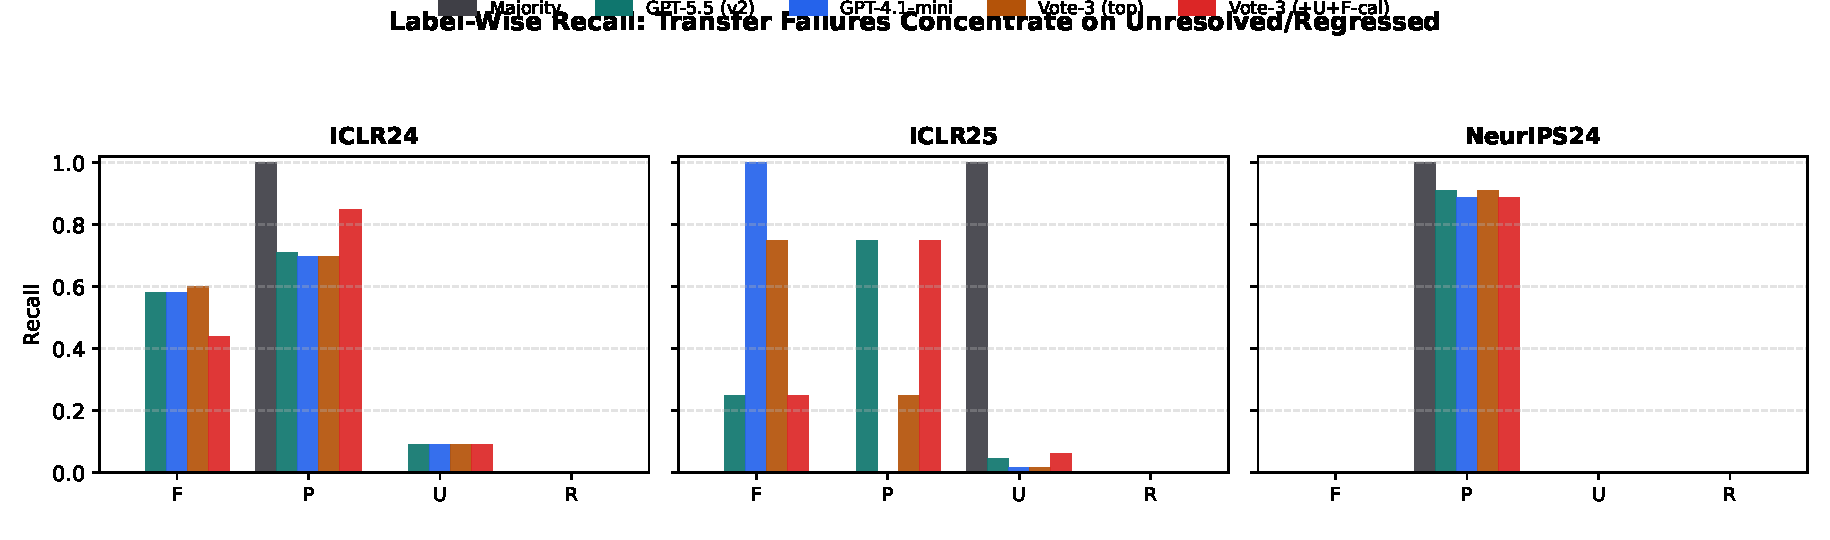
\includegraphics[width=\textwidth]{figures/figure4_prompted_llm_label_recall.pdf}
\caption{Label-wise recall for majority baseline, prompted LLMs, and vote ensemble. Cross-year failures are dominated by unresolved under-recovery and zero regressed recall under prompted transfer.}
\label{fig:prompted-llm-recall}
\end{figure*}

\begin{figure*}[t]
\centering
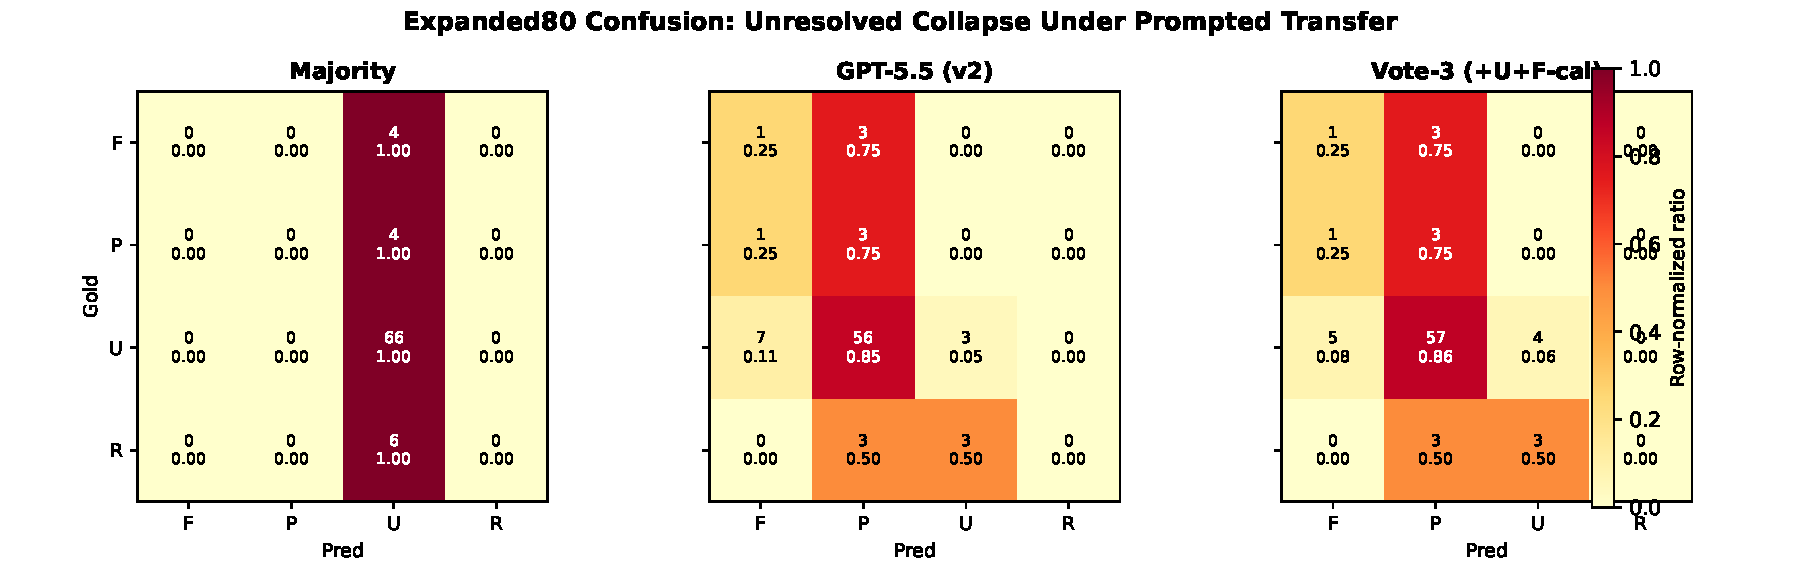
\includegraphics[width=\textwidth]{figures/figure5_expanded80_confusion.pdf}
\caption{Expanded80 row-normalized confusion matrices for majority baseline, GPT-5.5(v2), and Vote-3(+U+F-cal). Prompted transfer over-credits unresolved concerns as fixed/partial, while calibrated safeguards increase unresolved recovery but introduce additional tradeoffs.}
\label{fig:prompted-llm-confusion}
\end{figure*}

Figure~\ref{fig:prompted-llm-recall} explains why pooled prompted systems still fail under transfer.
In ICLR 2025 expanded80, prompted systems frequently over-credit unresolved cases as fixed or partial, so unresolved recall collapses to near-zero levels while regressed recall remains zero.
In NeurIPS limit100, the user-confirmed active frontier contains only partially-fixed and unresolved labels, and prompted models again collapse unresolved recall to zero by over-predicting partially-fixed.
Figure~\ref{fig:prompted-llm-confusion} localizes this failure in confusion space: most unresolved rows are reassigned to fixed/partial columns under prompted transfer.

\begin{figure*}[t]
\centering
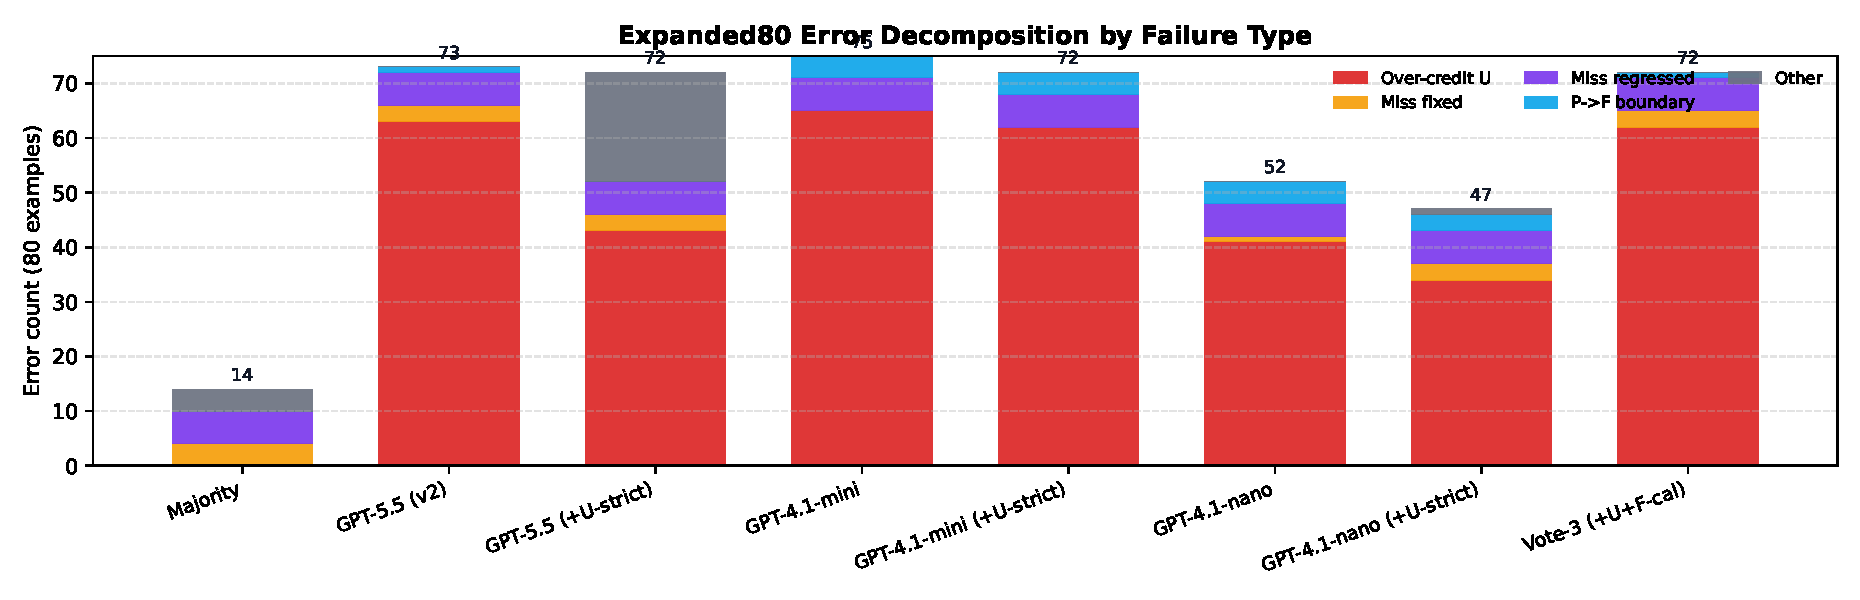
\includegraphics[width=\textwidth]{figures/figure6_expanded80_error_stack.pdf}
\caption{Expanded80 stacked error decomposition. Over-crediting unresolved concerns dominates all prompted variants; unresolved-strict prompting reduces this category for GPT-5.5, GPT-4.1-mini, and GPT-4.1-nano, but transfer brittleness remains.}
\label{fig:prompted-llm-error-stack}
\end{figure*}

Figure~\ref{fig:prompted-llm-error-stack} quantifies the same pattern at error-type granularity.
Across models, over-crediting unresolved concerns is the largest error bucket by a wide margin, while regression misses remain persistent.
These label-level failures explain why aggregate in-domain gains do not translate into robust transfer behavior.

\section{Discussion}

RevTrack suggests that review assistance should be evaluated as evidence tracking rather than static critique generation.
The practical failure mode is not merely that a model makes a wrong label.
It is that the model may keep repeating a criticism that has been fixed, or may credit a response that only defers the issue.
Both failures can distort author effort and reviewer attention.

The benchmark also changes how model progress should be read.
Small accuracy differences are not meaningful when most examples are partially fixed.
Macro-F1 and per-label recovery are closer to the scientific workload: fixed cases test whether stale criticism is retired, while unresolved cases test whether a model resists superficial reassurance.
The failure taxonomy makes this point concrete.
On the expanded ICLR 2025 frontier, many transfer errors are not random confusions; they are recognizable scientific-assistance failures such as over-crediting unresolved concerns, keeping fixed criticisms alive, and missing regressions.

The expanded ICLR 2025 frontier strengthens the cross-year story but also sharpens the boundary of the claim.
It confirms brittleness on a larger active frontier, yet the sample is deliberately hard and disagreement-heavy.
This is useful evidence for a benchmark paper because it shows where static matching breaks under pressure.
The NeurIPS active frontier and ICLR 2023 random/stratified slice broaden that evidence, but they still do not imply that the same label distribution holds across all venues or years.
A bounded independent second-pass mini60 check now provides reliability support, but the next step is still a non-ICLR random/stratified slice for broader prevalence-sensitive evidence.

More broadly, RevTrack points to a design requirement for scientific assistants.
They need an issue ledger: a structured representation of what was criticized, what evidence was added, and what status each concern should now have.
That representation is not a complete solution, but it gives the field a measurable target for longitudinal scientific judgment.

\section{Related Work}

\paragraph{Scientific peer review and review assistance.}
Peer-review datasets have enabled computational study of review text, scores, decisions, and reviewing workflows.
PeerRead introduced a public corpus of paper drafts, decisions, and expert reviews from venues including ACL, NeurIPS, and ICLR \citep{kang-etal-2018-dataset}.
NLPeer expands this line with a clearly licensed, multi-domain resource that includes drafts, camera-ready versions, reviews, metadata, and versioning information \citep{dycke-etal-2023-nlpeer}.
More recent resources such as Re2 collect full-stage review and rebuttal discussions across many OpenReview venues \citep{zhang-etal-2025-re2}.
Task inventories for peer-review automation also emphasize that reviewing decomposes into many different subtasks and that dataset documentation matters for comparability \citep{staudinger-etal-2024-analysis}.
Earlier automatic-review systems such as DeepReviewer and ReviewRobot also establish the paper-review automation line with score/comment generation objectives \citep{leng-etal-2019-deepreviewer,wang-etal-2020-reviewrobot}.
Recent LLM-era work extends this line with larger review datasets and staged reasoning pipelines for review generation \citep{zhu-etal-2025-deepreview}.
These resources provide the raw setting for studying scientific review, but their main tasks are usually paper-level prediction, review understanding, or discussion modeling.
RevTrack changes the unit of evaluation.
Rather than predicting acceptance, summarizing reviews, or modeling discussions wholesale, it isolates one reviewer concern and asks whether later revision evidence changes that concern's status.
This makes revision tracking closer to an issue ledger than to a static review corpus.

\paragraph{Review-question answering and evidence grounding.}
PeerQA uses peer-review questions as document-level scientific QA prompts and asks systems to retrieve evidence, identify unanswerable questions, and generate answers \citep{baumgartner-etal-2025-peerqa}.
RevTrack shares the emphasis on authentic reviewer information needs, but changes the output from answer generation to status tracking.
More broadly, evidence-verification benchmarks such as FEVER test whether claims are supported, refuted, or lack enough information with respect to textual evidence \citep{thorne-etal-2018-fever}.
RevTrack differs in two ways.
First, the claim is not a standalone fact: it is an old review concern whose status depends on later author response and revision evidence.
Second, the correct label is not only supported versus refuted.
Partial fixes and regressions are first-class outcomes because scientific revision often narrows, complicates, or worsens a concern rather than simply resolving it.
This perspective is also connected to QA with conflicting evidence, where systems must avoid over-confident answers when contexts disagree \citep{liu-etal-2025-open,shaier-etal-2024-adaptive}.

\paragraph{LLM-assisted reviewing.}
LLM-based review assistance has focused heavily on generating reviewer feedback.
Large-scale empirical work suggests that GPT-4 feedback can overlap with human-reviewer feedback and can be perceived as useful by authors \citep{liang-etal-2023-can}.
Targeted critique/meta-review assistance has also been studied directly for NLP papers \citep{du-etal-2024-llms-assist}.
At the same time, pilot evidence reports only limited net utility for generic peer-review assistance prompts \citep{robertson-2023-gpt4-helpful}.
For example, MARG uses multiple specialized LLM agents to generate scientific-paper feedback and reduce generic comments \citep{darcy-etal-2024-marg}.
This direction is useful, but review generation alone does not test whether an assistant can retire stale criticisms after a paper changes.
RevTrack therefore evaluates a narrower and more auditable capability: revision-aware issue tracking.
This framing also separates assistance quality from fluency.
A system can write a plausible comment while still failing the longitudinal decision of whether a prior comment should remain active.

\paragraph{Reliability, calibration, and hallucination under evidence conflict.}
LLM-as-judge methods have become common for scalable open-ended evaluation \citep{zheng-etal-2023-judging,liu-etal-2023-g}, and related work explores using panels of smaller judges to reduce cost and single-model bias \citep{verga-etal-2024-replacing}.
At the same time, LLM evaluators can show position and fairness biases that require calibration \citep{wang-etal-2024-large-language-models-fair}.
LLMs are also increasingly studied as data annotators or annotation assistants \citep{tan-etal-2024-large,gu-etal-2025-large}.
These lines motivate our prompted-LLM baselines, but they also make direct substitution of LLM labels for validated status labels risky.
Recent work has shown that strong language models can remain unreliable under factual pressure or conflicting evidence, even when outputs are fluent \citep{lin-etal-2022-truthfulqa,ji-etal-2023-hallucination-survey}.
Confidence-aware analyses also show that model certainty is not a sufficient proxy for correctness \citep{kadavath-etal-2022-language}.
This reliability gap under shift is consistent with broader calibration and robustness findings beyond review tasks \citep{guo-etal-2017-calibration,ovadia-etal-2019-shift,koh-etal-2021-wilds}.
Post-hoc hallucination checks can improve auditing \citep{manakul-etal-2023-selfcheckgpt}, but they do not directly solve the longitudinal decision in review workflows.
RevTrack complements this line by making the evaluation target explicit: whether a previously raised concern should stay active after revision evidence.

\paragraph{Evaluation under skew.}
The accuracy trap observed here is a standard risk in imbalanced classification, but it is especially damaging for review support.
The minority labels are often the scientifically important ones: fixed cases determine whether stale criticism should be retired, and unresolved cases determine whether a blocker remains active.
RevTrack therefore treats macro-F1, fixed-case recovery, unresolved-case recovery, and regressed-case analysis as part of the task definition rather than secondary diagnostics.

\section{Limitations}

The current strongest performance evidence is in-domain ICLR 2024.
The ICLR 2025 repro set is validated but small, and expanded80 plus NeurIPS 2024 limit100 are active frontiers rather than random or natural-prevalence samples.
The ICLR 2023 random80 slice adds random/stratified evidence within the ICLR venue family, but it is still standard single-user validation and not a full natural-prevalence estimate for all venues.
Most labels are standard single-user confirmed labels.
Second-pass reliability evidence is currently bounded to two packets: an independent mini60 packet and a broader boundary160 packet that was prelabel-assisted before user confirmation.
We therefore frame cross-year and cross-venue evidence as bounded transfer and external-validity evidence, not as a complete estimate of performance on all issues.
For the same reason, frontier failure-taxonomy counts should be read as diagnostic counts on intentionally hard frontiers, while random80 counts should be read by measured slice design rather than as broad prevalence estimates.
These agreement results should be interpreted narrowly: they are bounded consistency checks on hard cases, not a substitute for full two-annotator coverage across all packets.

The label rubric is issue-level and evidence-based, but some concerns remain ambiguous.
For example, a narrowed claim may make an original criticism less severe without fully resolving it.
These cases depend on careful evidence spans and notes.

The current labeled pool has too few regressed examples for stable regression-performance conclusions.
We include the label because it is conceptually important, but treat regression performance as provisional until more examples are collected.

RevTrack is also text-first.
The current pipeline uses review text, author responses, revision summaries, and available paper metadata rather than full PDF differencing.
This keeps the first benchmark auditable and lightweight, but it can miss changes that are only visible in figures, equations, or revised appendices.
Future versions should add PDF-aware evidence extraction while preserving issue-level provenance.

Finally, the current standard labels come from user-reviewed AI-assisted signoff and user-confirmed expanded80, NeurIPS 2024, and ICLR 2023 adjudication.
A separate independent mini60 second pass is complete, and a user-confirmed boundary160 second-pass packet is also complete.
Because boundary160 was prelabel-assisted, full-scale blind-independent two-annotator coverage remains future work.

\section{Ethics Statement}

RevTrack is built from public OpenReview discussions and is intended for evaluation and diagnostic research.
The benchmark should not be used to automate acceptance decisions or replace human reviewers.
Its appropriate use is to test whether research-assistant systems preserve scientific standards when helping authors or reviewers reason about revisions.

Because the data involves real papers and reviews, releases should preserve only necessary text snippets, document provenance, and follow venue policies.
We separate blind validation sheets from hidden assistant/model keys to reduce label leakage and to make audit boundaries explicit.
We do not release hidden assistant/model keys as human labels unless they have passed the documented promotion path.
The intended release artifact is therefore an audited benchmark package: minimally necessary text excerpts, labels with evidence spans, provenance metadata, scripts, and machine-readable audit reports, rather than a bulk mirror of full review discussions.


\bibliography{refs}

\appendix
\section{Audit and Reproducibility Details}

The current project artifacts include machine-readable reports for candidate-pool quality, human-validation packet integrity, label-evidence completeness, citation integrity, signoff quality, and paper-readiness status.
The paper-readiness audit reports status \texttt{ready} for the core claim set, with nine ready claims, zero blockers, and zero warnings.
The draft uses the public ACL style-file release \citep{aclstylefiles} and is aligned with the EMNLP 2026 main-conference call \citep{emnlp2026cfp}.

Table~\ref{tab:artifact-manifest} lists the paper-facing artifact manifest used to audit the current claim set.

\begin{table*}[t]
\centering
\scriptsize
\setlength{\tabcolsep}{3pt}
\begin{tabular}{p{0.13\textwidth}p{0.27\textwidth}p{0.34\textwidth}p{0.16\textwidth}}
\toprule
Artifact & Local file & Role in the paper & Current gate \\
\midrule
Readiness audit & \path{paper_readiness_audit.md} & Summarizes blockers, warnings, and claim readiness before paper use & ready; 0 blockers \\
Claim ledger & \path{claim_evidence_ledger.md} & Maps each paper claim to supporting metrics and counterevidence & 9 ready claims \\
Dataset card & \path{docs/revtrack_dataset_card_v0.md} & Records collection scope, provenance, label policy, and release boundaries & standard labels locked \\
Validation queue & \path{human_validation_work_queue.md} & Tracks all active standard validation packets and pending rows across ICLR, NeurIPS, and random/stratified lanes & 301/301 complete \\
Expanded80 transfer & \path{iclr2025_expanded80_standard_transfer_metrics.md} & Reports cross-year active-frontier transfer metrics with provenance caveats & standard-labeled frontier \\
Failure taxonomy & \path{failure_taxonomy.md} & Connects model errors to stale criticism, over-crediting, fixed under-recovery, and regression blindness & paper-facing analysis \\
Prompted LLM intervals & \path{prompted_llm_bootstrap_intervals.md} & Reports example-level bootstrap intervals for selected prompted LLM and vote baselines & stress evidence \\
NeurIPS transfer & \path{neurips2024_limit100_standard_transfer_metrics.md} & Reports user-confirmed cross-venue active-frontier transfer metrics & standard single-user active frontier \\
ICLR 2023 random80 & \path{iclr2023_limit80_random80_standard_transfer_metrics.md} & Reports bounded random/stratified external-validity evidence with provenance caveats & standard single-user slice \\
Citation audit & \path{paper_citation_audit.md} & Checks cited keys, BibTeX entries, required metadata fields, and final LaTeX citation warnings & pass; 26/26 keys resolved \\
\bottomrule
\end{tabular}
\caption{Repository artifact manifest for reproducibility and claim auditing. Paths are relative to the paper-asset or repository root as appropriate.}
\label{tab:artifact-manifest}
\end{table*}

\begin{table*}[t]
\centering
\scriptsize
\setlength{\tabcolsep}{3pt}
\begin{tabular}{p{0.12\textwidth}p{0.21\textwidth}p{0.21\textwidth}p{0.26\textwidth}}
\toprule
Work & Main artifact or task & Overlap & RevTrack distinction \\
\midrule
PeerRead \citep{kang-etal-2018-dataset} & Drafts, reviews, decisions, and score-prediction tasks & Scientific peer-review data & Tracks issue-level post-revision status rather than acceptance or score prediction \\
NLPeer \citep{dycke-etal-2023-nlpeer} & Licensed multidomain peer-review corpus with versioning & Versioned review data & Converts versioned context into concern-resolution labels with evidence spans and audits \\
Re2 \citep{zhang-etal-2025-re2} & Full-stage review, rebuttal, and discussion corpus & Reviewer-author interaction & Narrows whole discussions to one concern and one post-revision status label \\
PeerQA \citep{baumgartner-etal-2025-peerqa} & Peer-review questions for scientific QA & Reviewer information needs & Outputs revision status rather than generated answers \\
FEVER \citep{thorne-etal-2018-fever} & Evidence-grounded claim verification & Supported/refuted evidence reasoning & The claim is a historical review concern whose status can change after revision \\
MARG \citep{darcy-etal-2024-marg} & Multi-agent review-feedback generation & LLM assistance for reviewing & Evaluates retiring stale criticism, not generating new comments \\
\bottomrule
\end{tabular}
\caption{Adjacent benchmark and review-assistance settings compared with RevTrack.}
\label{tab:related-comparison}
\end{table*}

Table~\ref{tab:prompted-llm-postprocess-rules} reports an offline post-processing search on prompted-vote outputs.
The table is generated from machine-readable metrics in \path{postprocess_rule_search.json} to keep the calibration claim auditable.

\paragraph{Prompted LLM post-processing search.}
\begin{table*}[t]
\centering
\scriptsize
\setlength{\tabcolsep}{3pt}
\begin{tabular}{p{0.28\textwidth}rrrrr}
\toprule
Rule & Mean F1 & ICLR24 F1 & ICLR25 F1 & NeurIPS24 F1 & ICLR25 U Recall \\
\midrule
u\_guard\_fix\_suppress & 0.204 & 0.350 & 0.094 & 0.167 & 0.061 \\
u\_any & 0.202 & 0.345 & 0.092 & 0.170 & 0.061 \\
fixed\_suppress & 0.202 & 0.357 & 0.073 & 0.175 & 0.015 \\
base & 0.201 & 0.352 & 0.071 & 0.179 & 0.015 \\
\bottomrule
\end{tabular}
\caption{Offline post-processing rule search on top of a three-model prompted vote (GPT-5.5(v2), GPT-4.1-mini, Qwen2.5-72B). The best rule combines unresolved guarding with fixed-disagreement suppression.}
\label{tab:prompted-llm-postprocess-rules}
\end{table*}


\paragraph{In-domain significance check.}
Table~\ref{tab:iclr2024-significance} reports stratified-bootstrap confidence intervals and paired-bootstrap risk for the ICLR 2024 main results.
This is a split-level uncertainty check only: it does not model annotator uncertainty.
\begin{table}[t]
\centering
\scriptsize
\setlength{\tabcolsep}{3pt}
\resizebox{\columnwidth}{!}{%
\begin{tabular}{p{0.36\linewidth}rrrr}
\toprule
Model & Macro-F1 & 95\% CI & $\Delta$ to Structured & $P(\leq 0)$ \\
\midrule
Structured & 0.704 & [0.630, 0.775] & 0.000 & 1.000 \\
Structured (No Overrides) & 0.424 & [0.352, 0.494] & 0.280 & 0.000 \\
MPNet + LinearSVC & 0.389 & [0.320, 0.461] & 0.314 & 0.000 \\
ModernBERT + LinearSVC & 0.387 & [0.311, 0.464] & 0.317 & 0.000 \\
TF-IDF + LinearSVC & 0.376 & [0.305, 0.447] & 0.328 & 0.000 \\
Majority label & 0.184 & [0.184, 0.184] & 0.520 & 0.000 \\
\bottomrule
\end{tabular}
}
\caption{Stratified-bootstrap significance summary on ICLR 2024 clean dev v7. $P(\leq 0)$ is the paired-bootstrap probability that Structured is not better than the compared model on macro-F1.}
\label{tab:iclr2024-significance}
\end{table}


\paragraph{Cross-split significance check.}
Table~\ref{tab:cross-split-significance} extends the same bootstrap protocol to ICLR 2025 expanded80 and NeurIPS 2024 limit100 standard frontiers.
This check quantifies uncertainty under transfer difficulty and preserves the same no-IAA boundary.
\begin{table*}[t]
\centering
\scriptsize
\setlength{\tabcolsep}{3pt}
\begin{tabular}{p{0.24\textwidth}p{0.22\textwidth}rrrr}
\toprule
Split & Model & Macro-F1 & 95\% CI & $\Delta$ to anchor & $P(\leq 0)$ \\
\midrule
ICLR 2024 clean dev v7 & Structured (anchor) & 0.704 & [0.630, 0.775] & 0.000 & 1.000 \\
 & Structured (No Overrides) & 0.424 & [0.352, 0.494] & 0.280 & 0.000 \\
 & MPNet + LinearSVC & 0.389 & [0.320, 0.461] & 0.314 & 0.000 \\
 & ModernBERT + LinearSVC & 0.387 & [0.311, 0.464] & 0.317 & 0.000 \\
 & TF-IDF + LinearSVC & 0.376 & [0.305, 0.447] & 0.328 & 0.000 \\
 & Majority label & 0.184 & [0.184, 0.184] & 0.520 & 0.000 \\
\midrule
ICLR 2025 expanded80 standard frontier & Issue ledger (anchor) & 0.469 & [0.323, 0.577] & 0.000 & 1.000 \\
 & Structured & 0.298 & [0.218, 0.352] & 0.171 & 0.060 \\
 & MPNet & 0.276 & [0.140, 0.372] & 0.193 & 0.000 \\
 & Majority label & 0.226 & [0.226, 0.226] & 0.243 & 0.000 \\
 & ModernBERT & 0.092 & [0.054, 0.134] & 0.377 & 0.000 \\
 & TF-IDF & 0.026 & [0.025, 0.028] & 0.443 & 0.000 \\
\midrule
NeurIPS 2024 limit100 standard frontier & MPNet (anchor) & 0.348 & [0.299, 0.390] & 0.000 & 1.000 \\
 & Issue ledger & 0.211 & [0.173, 0.253] & 0.136 & 0.000 \\
 & Structured & 0.197 & [0.141, 0.250] & 0.150 & 0.000 \\
 & Majority label & 0.177 & [0.177, 0.177] & 0.170 & 0.000 \\
 & TF-IDF & 0.177 & [0.177, 0.177] & 0.170 & 0.000 \\
 & ModernBERT & 0.137 & [0.082, 0.193] & 0.211 & 0.000 \\
\bottomrule
\end{tabular}
\caption{Stratified-bootstrap macro-F1 confidence intervals across standard RevTrack splits. $P(\leq 0)$ is the paired-bootstrap probability that the split anchor is not better than the compared model.}
\label{tab:cross-split-significance}
\end{table*}


\paragraph{Prompted LLM uncertainty audit.}
Table~\ref{tab:prompted-llm-bootstrap} reports example-level bootstrap intervals for selected prompted LLM and vote baselines.
The intervals are used as a claim-risk check: they capture sample instability in the current splits, while leaving annotator uncertainty and API stochasticity as separate limitations.
\input{tables/prompted_llm_bootstrap_intervals}

\paragraph{Prompted LLM significance vs majority.}
Table~\ref{tab:prompted-llm-significance} reports paired stratified-bootstrap deltas against the majority baseline.
It strengthens the transfer-boundary statement with a direct hypothesis-test style view: prompted methods are significantly above majority in-domain, significantly below majority on ICLR25 expanded80, and overlapping on NeurIPS24.
\begin{table*}[t]
\centering
\scriptsize
\setlength{\tabcolsep}{3pt}
\begin{tabular}{llccccc}
\toprule
Dataset & Method & $n$ & Macro-F1 & $\Delta$ vs Majority & 95\% CI ($\Delta$) & $p(\Delta\le0)$ \\
\midrule
ICLR24 & GPT-5.5 (v2) & 148 & 0.350 & 0.167 & [0.093, 0.250] & 0.000 \\
ICLR24 & GPT-4.1-mini & 148 & 0.347 & 0.164 & [0.091, 0.245] & 0.000 \\
ICLR24 & Vote-3 (+U+F-cal) & 148 & 0.350 & 0.167 & [0.097, 0.244] & 0.000 \\
ICLR25 & GPT-5.5 (v2) & 80 & 0.081 & -0.145 & [-0.200, -0.068] & 1.000 \\
ICLR25 & GPT-4.1-mini & 80 & 0.066 & -0.160 & [-0.176, -0.136] & 1.000 \\
ICLR25 & Vote-3 (+U+F-cal) & 80 & 0.094 & -0.132 & [-0.198, -0.047] & 0.999 \\
NeurIPS24 & GPT-5.5 (v2) & 80 & 0.171 & -0.006 & [-0.019, 0.004] & 0.862 \\
NeurIPS24 & GPT-4.1-mini & 80 & 0.181 & 0.003 & [-0.012, 0.018] & 0.319 \\
NeurIPS24 & Vote-3 (+U+F-cal) & 80 & 0.167 & -0.011 & [-0.024, 0.001] & 0.966 \\
\bottomrule
\end{tabular}
\caption{Prompted LLM paired stratified-bootstrap significance against the majority baseline on standard-labeled splits. $\Delta$ is macro-F1(method) minus macro-F1(majority).}
\label{tab:prompted-llm-significance}
\end{table*}


\paragraph{Oral/rebuttal evidence panel.}
Table~\ref{tab:oral-evidence-panel} summarizes the highest-signal checkpoints used in oral/rebuttal discussion: in-domain gain, accuracy-trap evidence, transfer-frontier brittleness, prompted-significance boundary, mini-slice IAA reliability, and readiness-gate status.
\input{tables/oral_evidence_panel}

\paragraph{Representative oral casebook.}
Table~\ref{tab:oral-casebook-summary} lists representative failure cases used in oral Q\&A.
It complements aggregate metrics with concrete issue-level failure behavior for stale criticism, over-crediting unresolved concerns, fixed under-recovery, regression blindness, and partial/full-boundary errors.
\begin{table*}[t]
\centering
\scriptsize
\setlength{\tabcolsep}{3pt}
\begin{tabular}{p{0.18\textwidth}p{0.16\textwidth}p{0.13\textwidth}p{0.44\textwidth}}
\toprule
Failure mode & Split / model & Gold / prediction & Why it matters \\
\midrule
stale\_criticism & ICLR24 signoff / - & F / T:P, S:P & This example separates revision-aware judgment from static semantic plausibility. \\
accuracy\_trap\_fixed\_cases & ICLR25 repro / TF-IDF & F / T:P, S:P & This is the core reason the paper reports macro-F1 and per-label recovery. \\
over\_crediting\_unresolved & ICLR25 exp80 / Structured & U / T:P, S:F & This is the practical stale-assistant failure: the model would stop tracking an unresolved concern. \\
fixed\_under\_recovery & ICLR25 exp80 / TF-IDF & F / T:P, S:F & This motivates fixed-case F1 rather than accuracy-only reporting. \\
regression\_blindness & ICLR25 exp80 / TF-IDF & R / T:P, S:F & This justifies keeping the regressed label while avoiding strong regression-performance claims. \\
partial\_vs\_fixed\_boundary & ICLR25 exp80 / Ledger & P / T:P, S:P & This is the central label-boundary risk for benchmark reliability. \\
\bottomrule
\end{tabular}
\caption{Representative failure cases used for oral/rebuttal discussion.}
\label{tab:oral-casebook-summary}
\end{table*}


\paragraph{Worked issue-level examples.}
Table~\ref{tab:worked-issue-examples} provides compact concern/evidence snippets for one example each of \textit{fixed}, \textit{partially\_fixed}, \textit{unresolved}, and \textit{regressed}.
It is intended as a boundary-interpretation aid for readers and reviewers, not as a prevalence table.
\begin{table*}[t]
\centering
\scriptsize
\setlength{\tabcolsep}{3pt}
\begin{tabular}{p{0.10\textwidth}p{0.12\textwidth}p{0.34\textwidth}p{0.34\textwidth}}
\toprule
Gold label & Issue ID & Concern snippet & Response/revision evidence snippet \\
\midrule
fixed & \texttt{w7P92BEsb2\_\_r01} & Reviewer asks for concrete computational-cost comparison and questions whether efficiency claims are substantiated. & Revision adds direct cost/error comparisons (Figure 6; lines 510--530), satisfying the original evidence request. \\
partially\_fixed & \texttt{9k0krNzvlV\_\_r02} & Reviewer questions the practical contribution to open-model watermarking and asks for stronger empirical support. & Revision adds sample-efficiency plots, multi-key experiments, and clearer framing, but does not fully close the contribution concern. \\
unresolved & \texttt{My7lkRNnL9\_\_r01} & Reviewer asks whether one-hidden-layer theory can extend to deeper networks. & Author response acknowledges the limitation and adds discussion, but no new theory or decisive evidence resolves the core concern. \\
regressed & \texttt{VNMJfBBUd5\_\_r04} & Reviewer flags ambiguity and formulation issues in gradient-circular-distance definitions and layer-wise computation. & Revised response introduces additional explanation, but adjudication marks the issue as worsened/contradicted under the benchmark rubric, so the status remains regressed. \\
\bottomrule
\end{tabular}
\caption{Worked issue-level adjudication examples with concern and evidence snippets. These examples complement aggregate metrics and make label boundaries explicit.}
\label{tab:worked-issue-examples}
\end{table*}


\paragraph{Bounded second-pass reliability check.}
For a separate independent mini60 packet, second-pass labels are complete (60/60) with agreement $=1.0$, Cohen's $\kappa=1.0$, and zero mismatches.
This artifact is tracked in \path{iaa_second_annotator_mini60_v1_metrics.json} and surfaced by the readiness gate as bounded reliability evidence rather than full-scale two-annotator coverage.


\end{document}
